\documentclass[a4paper, 10pt, oneside]{book}
\usepackage[top=25mm, left=25mm, right=20mm, bottom=25mm]{geometry}
\usepackage[english]{babel}
\usepackage[T1]{fontenc}
\usepackage[utf8]{inputenc}
\usepackage{fancyhdr}
\usepackage{graphicx}
\usepackage{hyperref}
\usepackage{pstricks}
\usepackage{pst-node} % For connecting of onformation
\usepackage{auto-pst-pdf}

\newcommand{\DocumentVersion}{Version 0.01}
\newcommand{\DocumentName}{QFM Screen Sequence}

% Header definitions
\pagestyle{fancy} % Use fancy style
%\renewcommand{\headheight}{15.0pt}
\renewcommand{\footrulewidth}{0.4pt}
\fancyhf{}
\fancyhead[C]{\DocumentName}
\fancyhead[R]{\DocumentVersion}
\fancyhead[L]{-----Draft-----}
\fancyfoot[C]{\thepage}

\begin{document}
%\frontmatter
\setcounter{chapter}{0}
\begin{titlepage}
	\hypersetup{pageanchor=false}
	\center
	\vspace{1.5cm}
	{\huge\bfseries \DocumentName \par}
	\vspace{2cm}
	{\Large\itshape Heinrich Weinz\par}
	\vspace{1cm}
	{\large\itshape \DocumentVersion\par}
	\vfill
	{\large \today\par}
\end{titlepage}
\tableofcontents \newpage
%\mainmatter
\chapter{Frame sequence} \newpage
\centering
\begin{psmatrix}[rowsep=.5,colsep=.5]	
\rput[c](0,0){\rnode{Start}{\pscirclebox{\hyperlink {meinstart}{Start}}}}
\rput[c](0,-4){\rnode{StartScreen}{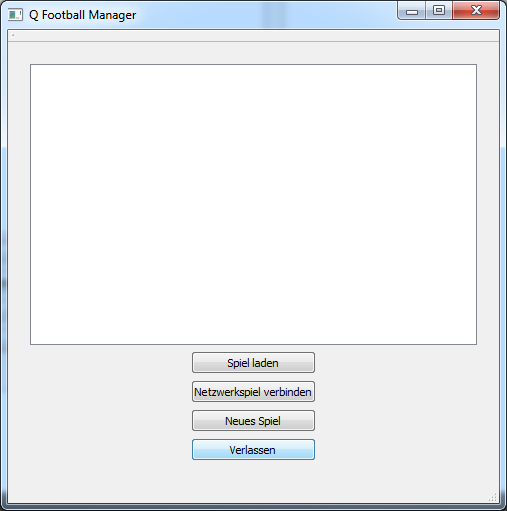
\includegraphics[scale=0.35]{Screens/StartScreen.png}}}
\rput[c](-7,-4){\rnode{StartQuit}{\pscirclebox{Quit}}}
\rput[c](4,-8){\pscirclebox{Loadbox}}
\end{psmatrix}
\ncline{->}{Start}{StartScreen}
\ncline[arcangle=-15]{<-}{StartQuit}{StartScreen}\naput[nrot=:U]{Quit button pressed}

\end{document}